\documentclass[11pt, fleqn]{article}

\usepackage{booktabs} % To use /toprule /midrule /bottomrule commands in printing tables
\usepackage{amsmath}
\usepackage{amsfonts}
\usepackage[margin=1in]{geometry} % To set the margin widths
\usepackage{graphicx}
\usepackage{multirow}
\usepackage{tabularx}
\usepackage{tikz}
\usepackage{varioref}

\setlength{\parskip}{12pt} % Sets a blank line in between paragraphs
\setlength\parindent{0pt} % Sets the indent for each paragraph to zero

\begin{document}

\title{Big Data: HW1}
\author{Will Clark, Matthew DeLio}
\date{\today}
\maketitle

\section{Data Visualization}

\begin{figure}[!htb]
  \centering
  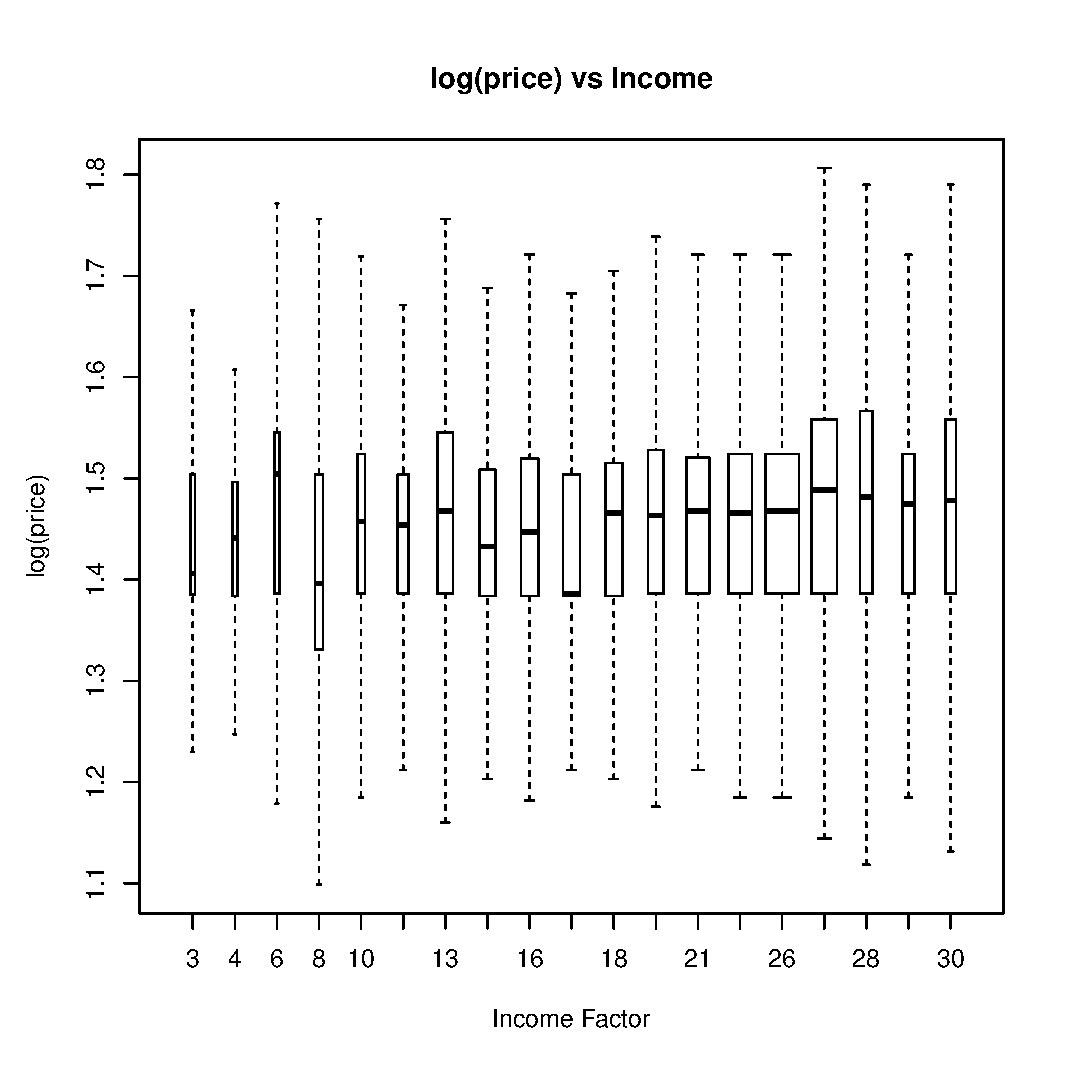
\includegraphics[scale=.5]{income.eps}
  \caption{Log of price by Income Classification}
  \label{fig:income}
\end{figure}

\begin{figure}[!htb]
  \centering
  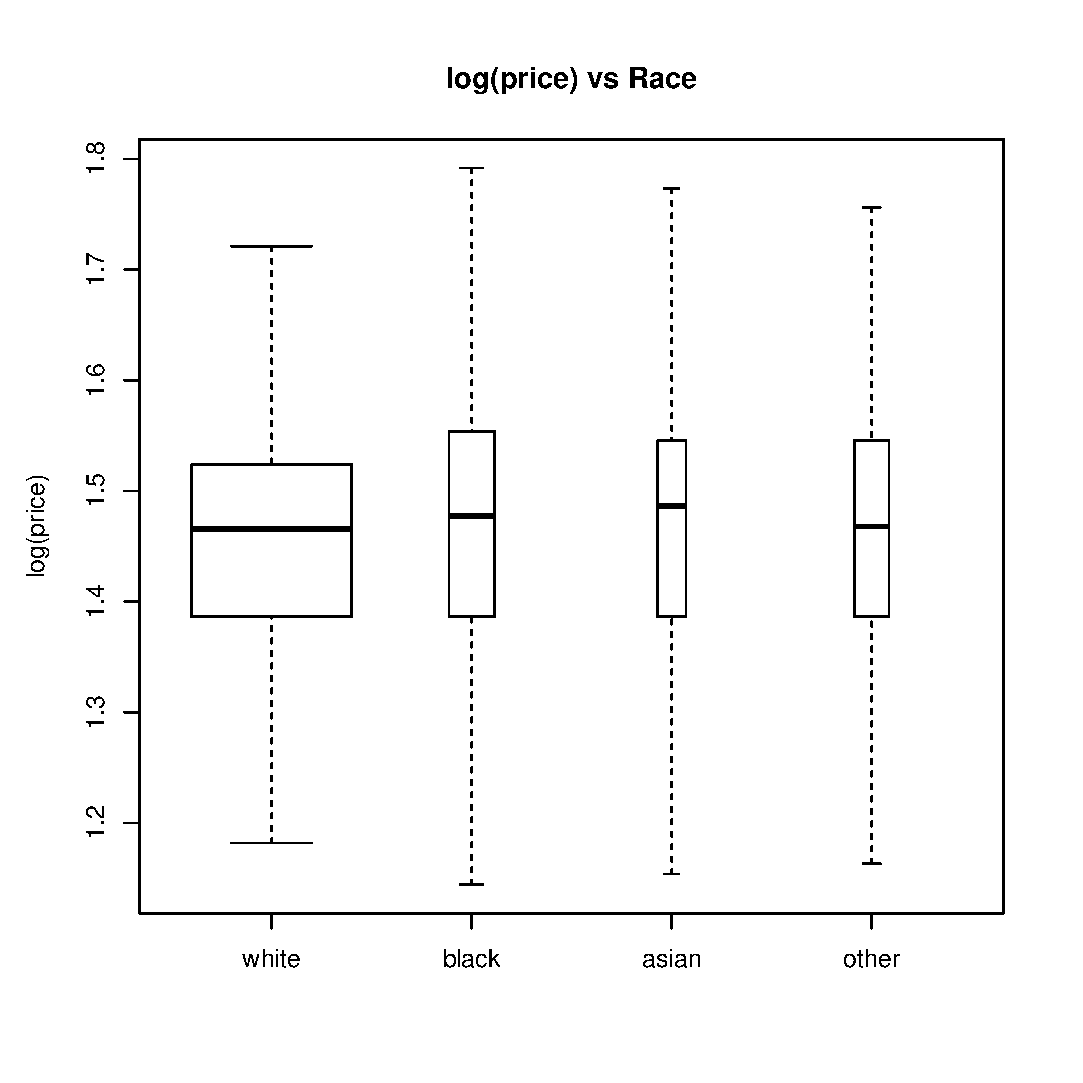
\includegraphics[scale=.5]{race.eps}
  \caption{Log of price by Race}
  \label{fig:race}
\end{figure}

\begin{figure}[!htb]
  \centering
  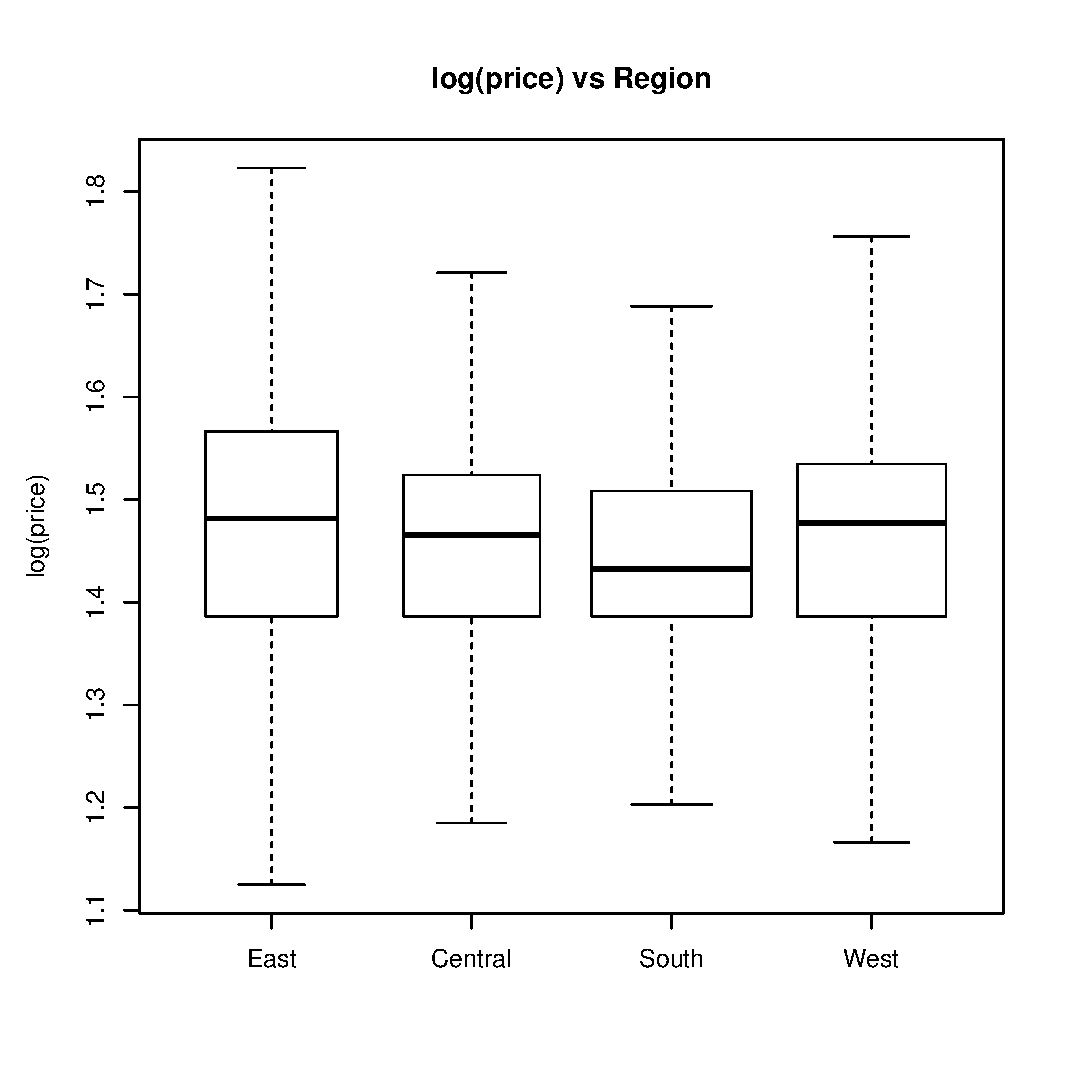
\includegraphics[scale=.5]{region.eps}
  \caption{Log of price vs. Region}
  \label{fig:region}
\end{figure}

Figure~\vref{fig:income} shows the relation between customers' income factor and $log(price)$.  Roughly speaking, customers are paying the same amount.  However, there is a slight increase in the median price for customers with higher levels on income.  This may indicate that coupon redemption is lower, or, alternatively, that higher income people shop for ice-cream in shops that charge more for products in general.

Figure~\vref{fig:race} shows the relation between race and $log(price)$.  From these data we see there most races are paying the same price for ice-cream.  If anything, the median price paid by the ``white'' population is slightly lower.

Figure~\vref{fig:region} shows the relation between geographic regions and $log(price)$.  These data indicate that the East Coast pays more for ice-cream than the rest of the country.  This may just by a proxy for a higher cost-of-living on the East Coast, or, alternatively, that the East Coast has higher demand for Ben and Jerry's ice-cream which is being capitalized on.

\section{Baseline Regression Model and Improvements}

The dependent variable is the log of price paid per unit of ice cream purchased. Independent variables describe:
\begin{itemize}
  \item flavor and size of unit purchased
  \item household demographics (size, income, marital status, race) and type (single family home or not)
  \item coupon use
  \item geographic region
  \item household appliances (microwave, dishwasher) and amenities (internet, cable TV)
\end{itemize}

One issue with this regression is that it includes many independent variables that co-vary highly with each other, which can make the estimates of each coefficient inaccurate. Specifically:
\begin{itemize}
  \item being married correlates highly with household income and household size (0.402 and 0.499, respectively);
  \item there are two variables for coupon use (each contains similar information);
  \item there are two variables to keep track of race (the second tracks Hispanic origin which is almost redundant given the classifications of the first)
\end{itemize}
Removing these redundant variables should increase the accuracy of the estimated coefficients for the remaining variables. 

There is also a risk of identifying false positives given that there are a large number of proposed explanatory variables. Using the Benjamini Horchberg algorithm, we find that to ensure a false positive rate of 1 percent or less, we should only accept p-values less than 0.0022.

There are tractability issues with the high number of flavors that are used as explanatory variables. By grouping the flavors into a popular group (the five most purchased) and an other group, we find that being a popular or unpopular flavor is not a significant predictor of purchase behavior (the p-values are greater than 0.0022).  A histogram of the pvalues after grouping the flavors and eliminating redundant variables is shown in Figure~\vref{fig:pvalue}.

\begin{figure}[!htb]
  \centering
  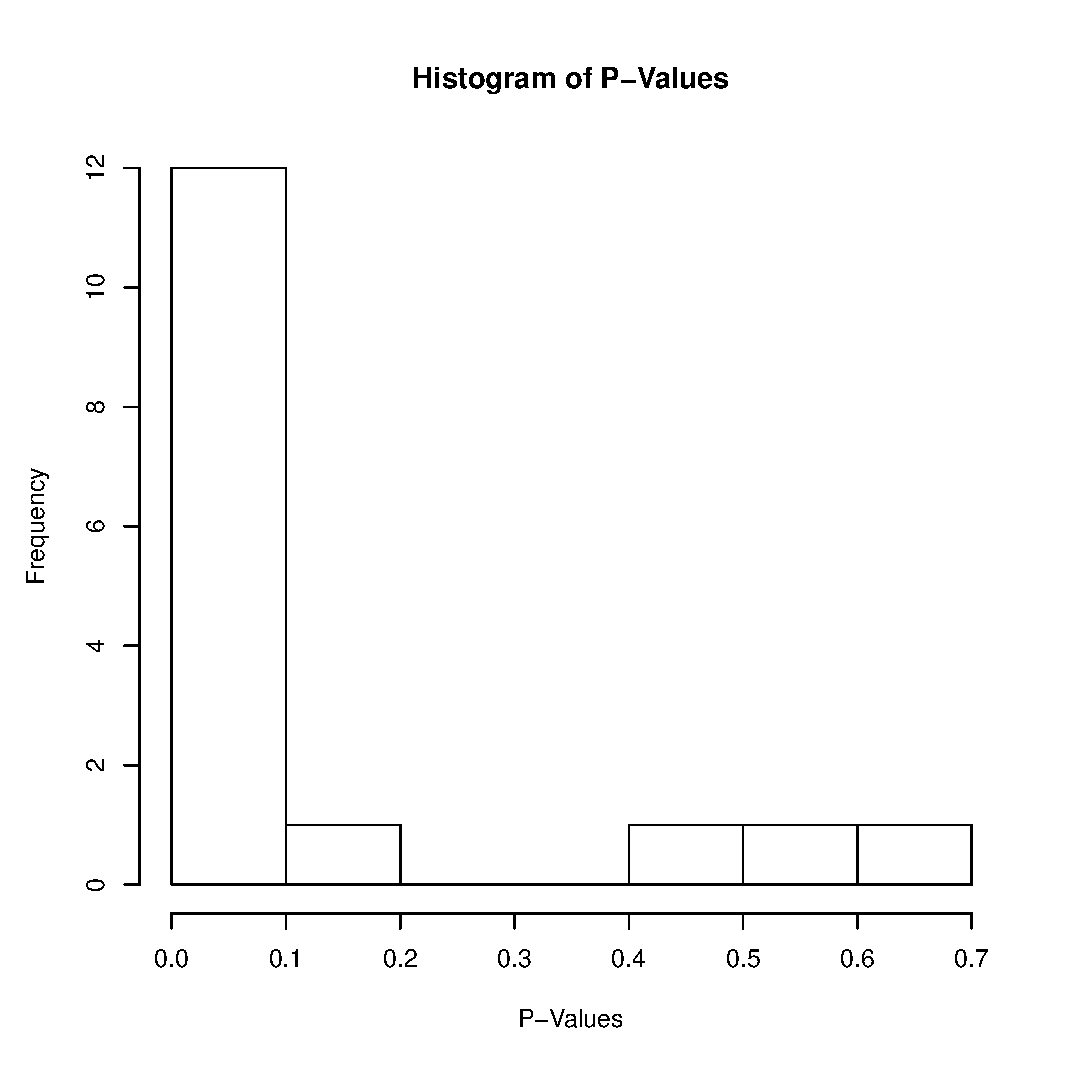
\includegraphics[scale=.5]{pvalue_hist.eps}
  \caption{P-value Histogram}
  \label{fig:pvalue}
\end{figure}

\section{Our Regression Model}

We omit variables with high col-linearity and include only variables that the B-H algorithm identifies as significant. The results from our final regression are presented in Table~\vref{tab:regress}.

\begin{table}
  \begin{tabular}{l r r r r l}
    \toprule
    Variable            & Estimate  & Std. Error &  t value  & p value & \\
    \midrule
    (Intercept)           & 1.4783538 & 0.0084187 & 175.604 & $<2e-16$ & ***\\
    size1\_descr32.0 MLOZ  & 0.3116734 & 0.0079110 & 39.397 & $<2e-16$ & *** \\
    household\_income      & 0.0019301 & 0.0001904 & 10.138 & $<2e-16$ & *** \\
    regionCentral         & -0.0215774 & 0.0031313 & -6.891 & 5.69e-12 & ** \\
    regionSouth           & -0.0263582 & 0.0029483 & -8.940 & $<2e-16$ & *** \\
    regionWest            & -0.0191600 & 0.0030068 & -6.372 & 1.90e-10 & *** \\
    household\_size        & -0.0062190 & 0.0008036 & -7.739 & 1.05e-14 & *** \\
    microwaveTRUE         & -0.0423604 & 0.0076230 & -5.557 & 2.78e-08 & *** \\
    sfhTRUE               & -0.0099485 & 0.0024945 & -3.988 & 6.68e-05 & *** \\
    usecoupTRUE           & 0.0107800 & 0.0032904 & 3.276 & 0.00105 & **  \\
    raceblack             & 0.0130186 & 0.0040255 & 3.234 & 0.00122 & **  \\
    raceasian             & -0.0035321 & 0.0063275 & -0.558 & 0.57670 & \\
    raceother             & 0.0161162 & 0.0051862 & 3.108 & 0.00189 & **  \\
    tvcableTRUE           & 0.0068942 & 0.0021707 & 3.176 & 0.00150 & **  \\
    \midrule
    \multicolumn{6}{l}{*** Significant at 99 percent level}\\
    \multicolumn{6}{l}{** Significant at 95 percent level}\\
    \bottomrule
  \end{tabular}
  \caption{Explanatory Variables}
  \label{tab:regress}
\end{table}

Some noteworthy conclusions from the regression:
\begin{itemize}
  \item Buying ice cream in larger sizes increase per unit consumption (spending increases 31 percentage points for every additional 32 oz purchased)
  \item Higher household income increases ice cream purchases;
  \item People spend more on ice cream in the East region than in any other region;
  \item Spending on ice cream falls as household size increases;
  \item Having a coupon increases spending on ice cream;
  \item Black and other races spend more on ice cream that white people (we cannot draw conclusions about Asian spending due to statistical insignificance);
  \item Households with cable TV spend more on ice cream than those without; households with a microwave spend less than those with one.
\end{itemize}

While all of these relationships are statistically significant, many of them are quite small. For example, moving up one category in the household income measure (typically an increase of \$5000) only increase ice cream expenditure by 0.2 percent.

In our application of the B-H algorithm, we required a false discovery rate of 1 percent. This implies that it is more likely than not that we do not have any false discoveries in this sample of 13 explanatory variables. Some variables, however, do not have any intuitive explanations (why should microwave ownership affect ice cream expenditures?) which leads us to believe that there may still be false positives among the set of explanatory variables.

\end{document}
